% Main chapter title
\chapter{Restricting Malicious Intent of Application}
\label{ch:current}

% This is for the header on each page
\lhead{Chapter 6. \emph{Restricting Malicious Intent of Application}}
\thispagestyle{empty}
Android current security system is based on the permissions. If an application needs to access any sensitive data or sensors which is considered as dangerous, then they need permissions to do that. In current security scenario, we can restrict the particular permission of an application. But major problem with current scenario is if we restrict the particular permission of an application, then application will not work properly as shown in Figure \ref{fig:prob1}.
\begin{figure}[h]
	\centering
	\begin{subfigure}[h]{0.45\textwidth}
		\centering
		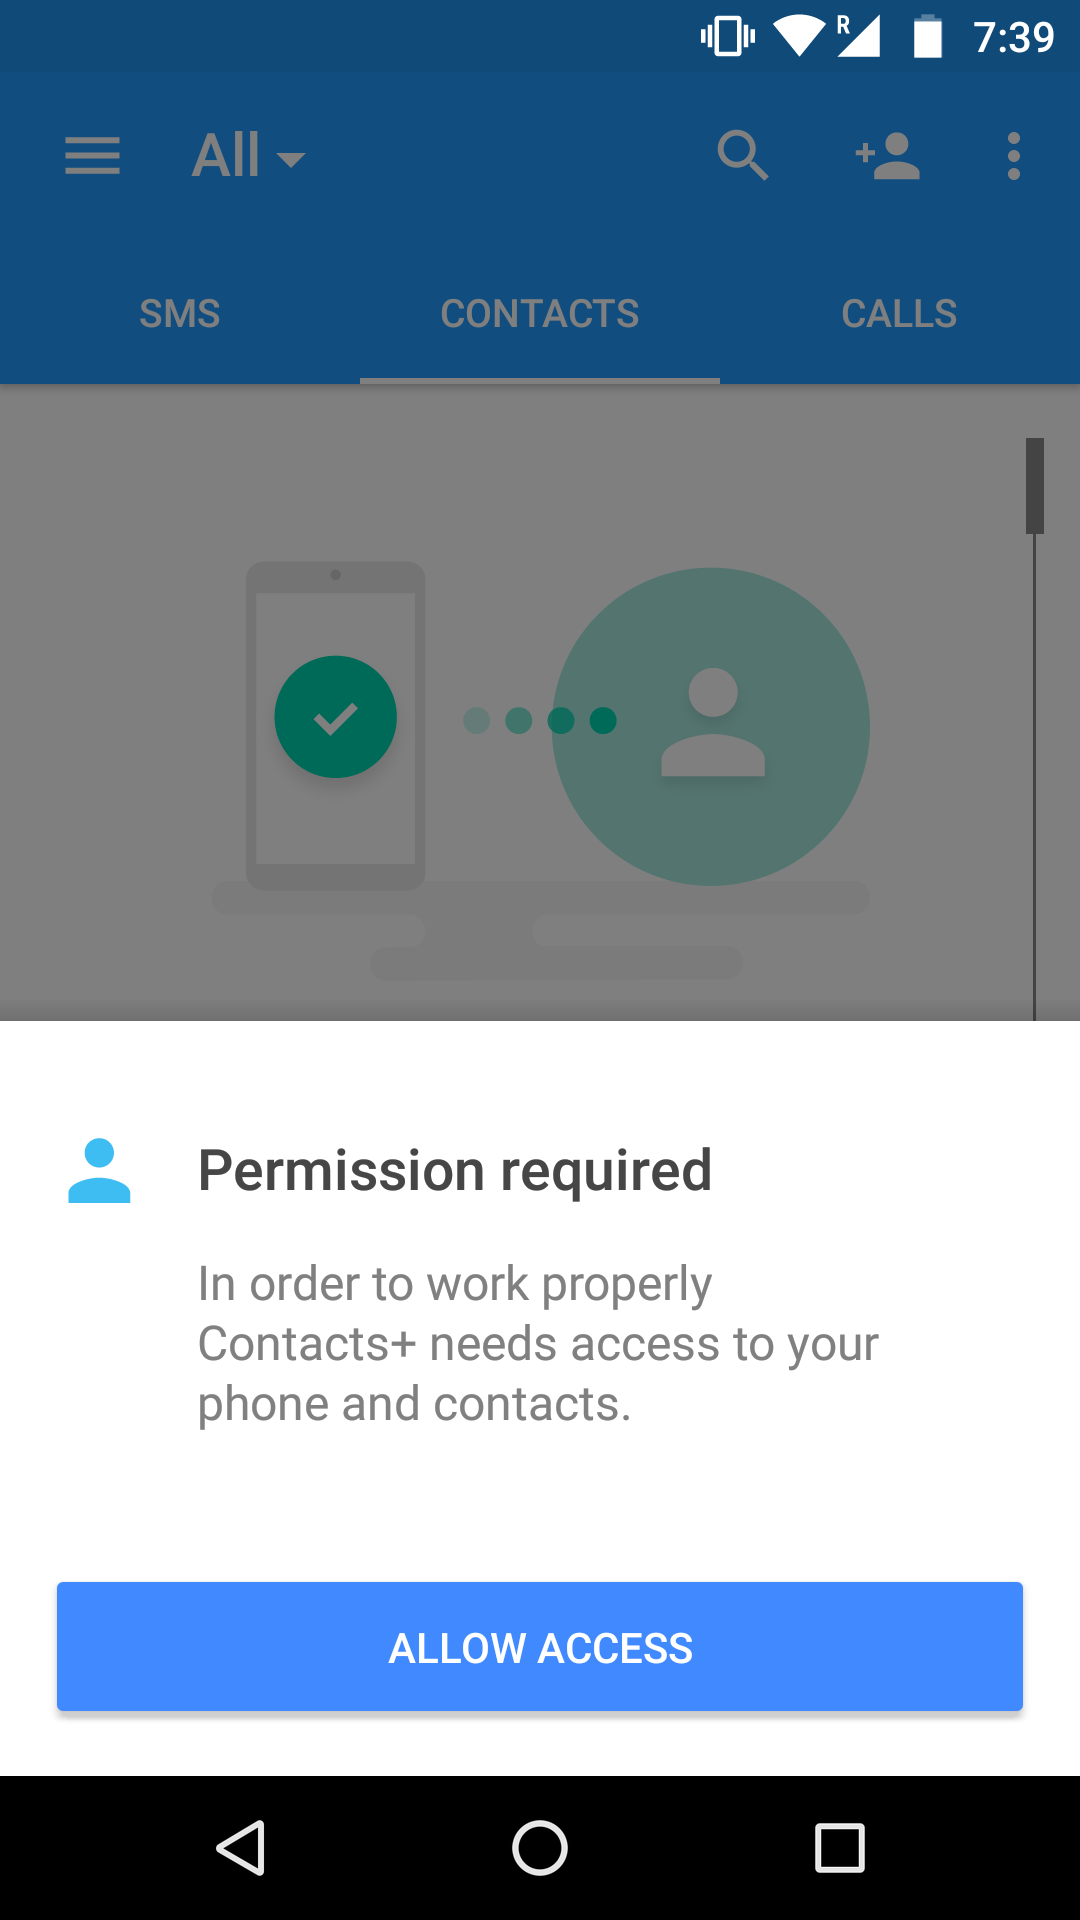
\includegraphics[width=\textwidth]{restrict_prob1.png}
		\caption{When permission to access phone is denied.}
	\end{subfigure}
	\hfill
	\begin{subfigure}[h]{0.45\textwidth}
		\centering
		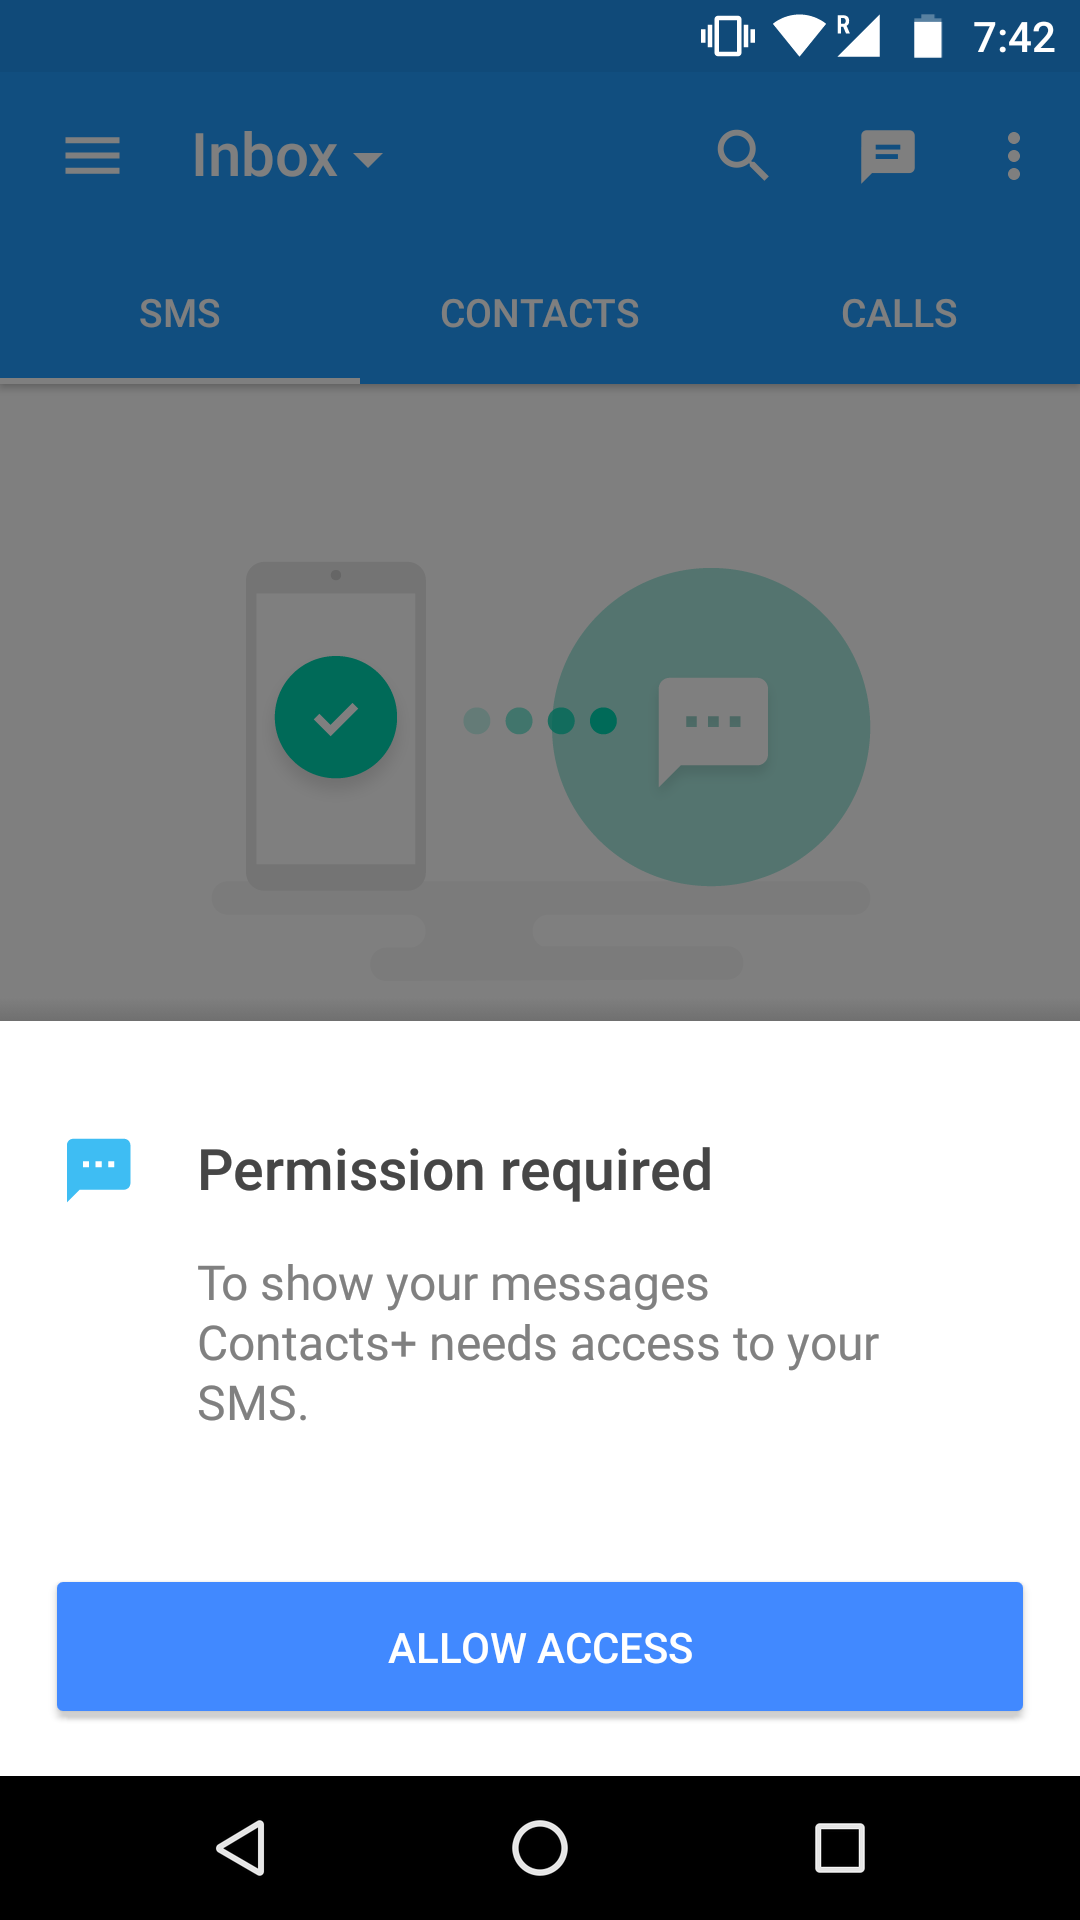
\includegraphics[width=\textwidth]{restrict_prob2.png}
		\caption{When permission to access message is denied.}
	\end{subfigure}
	\caption{Problems in Android current security scheme}
	\label{fig:prob1}
\end{figure}

Apart from the permissions, there are more things that can be used to exploit the private data of user and also can be used to degrade the performance of the device itself. Some of those are clipboard, view, etc. Clipboard is buffer which is used to hold the data copied from any application. Since clipboard is accessible to all applications, any application can read the data from clipboard and can send it to third party server. Currently, we can to stop applications from accessing clipboard data. Some applications opens the browser via link. We can stop link from opening in the browser.

Currently if an application asks permission to access message, then application will get permissions for both send message and read message. If we want to restrict an application such that it can read message but can not send. In other words, we want to control the permission of application at API level. But currently this feature is not provided by Android operating system.

We have to restrict the malicious behaviour of applications. Since, currently every application runs in its own process, with its own instance of the Dalvik virtual machine (DVK)/ Android runtime (ART). So, we can not restrict applications by developing another at fifth layer of the Android software stack. One way to restrict the malicious behaviour of applications is by modifying the Android Package (APK) file. For modifying the APK file, we have to decompile it and it convert it into smali and then we can change code of application. Smali is more of assembly based language so making change in smali is tedious task. Another way to restrict applications is without modifying the APK file. We can restrict applications at the system level by modifying the Random access memory (ROM). We have used Xposed framework \cite{xposedframework} to achieve this.\\ \\
\section{Wrapping Applicaitons}
Xposed is framework for module which can restrict or change the behaviour of the system and applications without touching any APKs. Xposed works at system level so your device should be rooted. Instead of modifying corresponding DEX or ART representation of the application, it is deeply integrated with the Android system where it replaces some system components after backing up the originals. There are multiple advantages to this approach. Some of them are:
\begin{itemize}
    \item you can modify parts of the system you otherwise could not.
    \item you can apply multiple modifications to the same app in a combination best fitting your intentions.
    \item changes are easy to undo: As all changes are done in the memory, you just need to deactivate the module and reboot to get your original system back.
\end{itemize}

Zygote is the main process of the Android runtime. Every application is started as  a copy (``fork") of it. So, this process is also called as the head of Android runtime. This process is started by an \textit{/int.rc} script when your phone is booted. The process is done with \textit{/system/bin/app\_process}, which loads the needed classes and invokes the initialization methods.

\begin{figure}[h]
	\centering
	\begin{subfigure}[h]{0.45\textwidth}
		\centering
		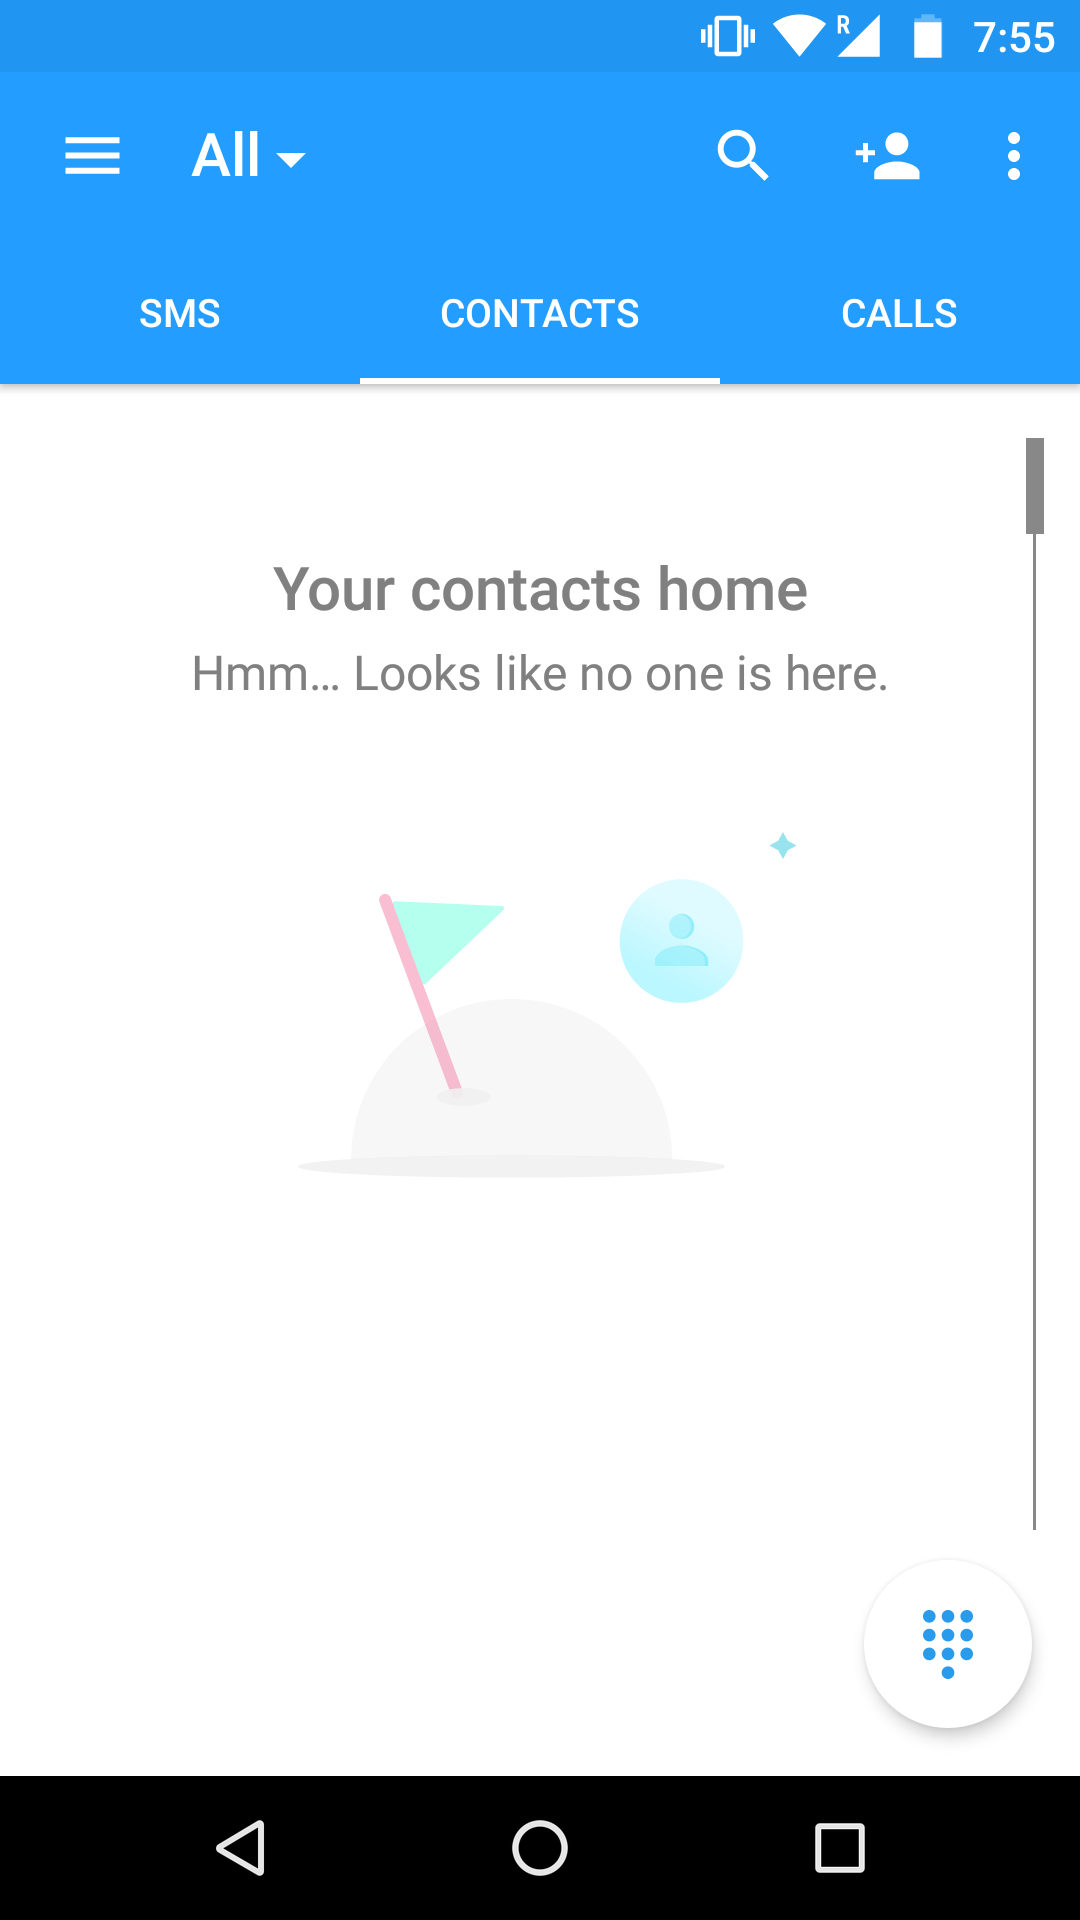
\includegraphics[width=\textwidth]{restrict_sol1.png}
		\caption{When permission to access phone is denied.}
	\end{subfigure}
	\hfill
	\begin{subfigure}[h]{0.45\textwidth}
		\centering
		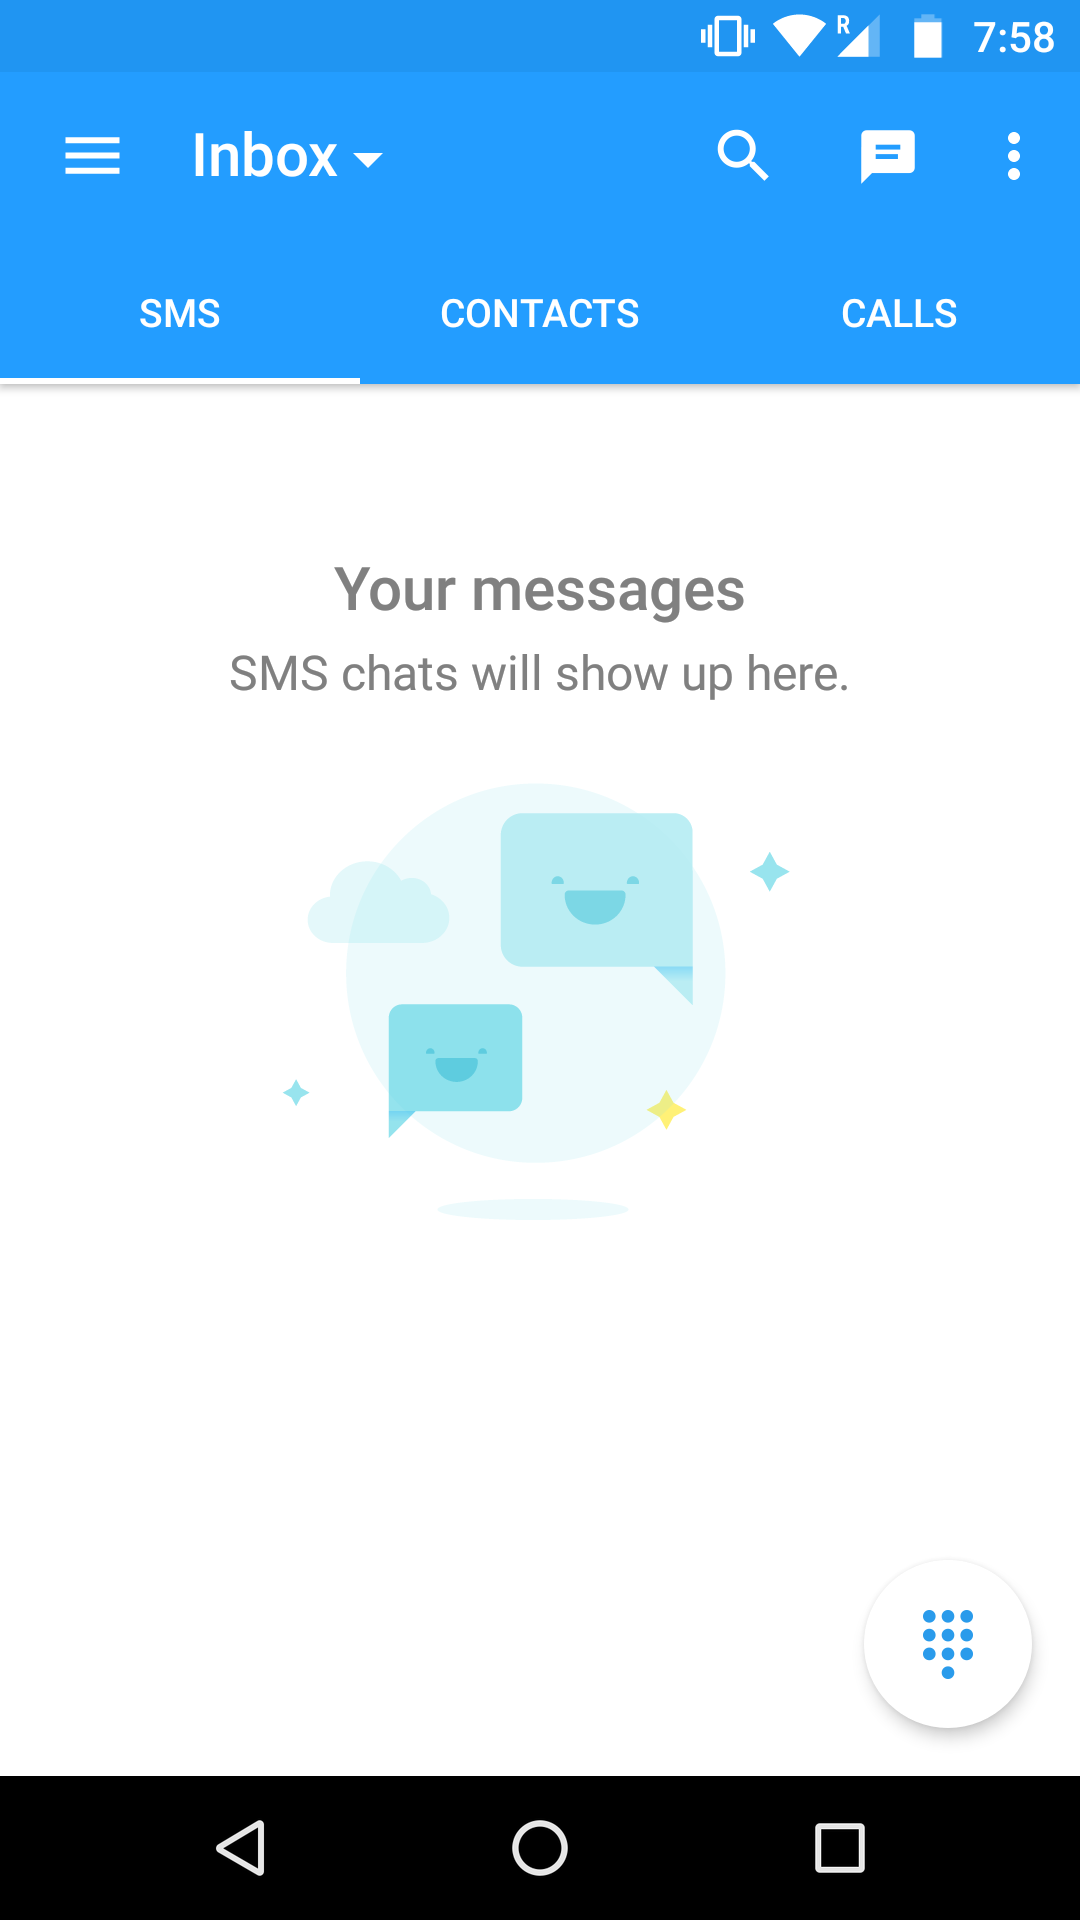
\includegraphics[width=\textwidth]{restrict_sol2.png}
		\caption{When permission to access message is denied.}
	\end{subfigure}
	\caption{App working properly after restrictions}
	\label{fig:prob2}
\end{figure}

Xposed framework creates an extended version of existing app\_process. When you install the framework, a modified and extended app\_process is copied to \textit{/sytem/bin}. This extended startup process adds an additional jar to the classpath and calls methods from there at certain places. For instance, just after the VM has been created, even before the main method of Zygote has been called. And inside that method, we are part of Zygote and can act in its context. So, now we can control
the method calls of other application from there.

To provide the security, we have to restrict the method calls from the application. When an application calls any method, we can do three things with that method. Either we can change the parameter of method or we can change body of the method. We can also leave the method unmodified. We have modified the existing modules of Xposed framework to control the methods. Now, if an application wants to access the resource, then we can feed the application with no data of fake data. We have restricted the applications from accessing contacts and messages. Since Xposed module does not revoke or block permissions from an application, so most application will continue to work as before and won't force close or crash as shown in Figure \ref{fig:prob2}. Now, we can also control the applications at API level. We can also restrict the application from pasting the data from clipboard either manually or automatically.
\section{Implementation}
Android provides different layers of software stack to handle different things. Currently, if an application invokes any methods, it is handled by Binder IPC module. Binder IPC module binds the method with native libraries. Interaction between apps, application framework, and linux kernel on Android is shown in Figure \ref{fig:impl1}.
\begin{figure}[!h]
  \centering
  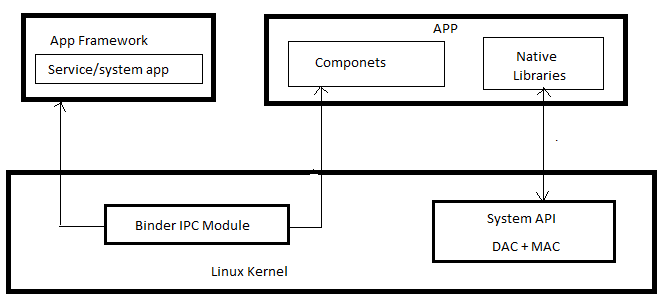
\includegraphics [scale=0.8] {impl1.png}
  \caption{Interaction between apps, application framework, and Linux kernel on Android}
  \label{fig:impl1}
\end{figure}

Xposed framework modifies the \textit{app\_process} file of \textit{/sytem/bin} and adds an extra jar file to Android to intercept the methods. Since, it modifies the \textit{app\_process} and every other process is child process of \textit{app\_process}, so Xposed becomes the integral part of the every methods. Workflow of Xposed framework is shown in Figure \ref{fig:impl2}.
\begin{figure}[!h]
  \centering
  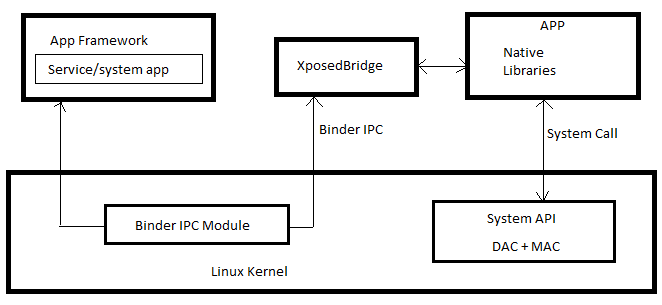
\includegraphics [scale=0.8] {impl2.png}
  \caption{Interaction between apps, application framework, and Linux kernel on Android}
  \label{fig:impl2}
\end{figure}

Xposed framework provides mechanism to intercept method calls of any application. Xposed provides \texttt{handleHookedMethod} to handle the methods call of applications. Using this method we can modify the parameters of method, or body of methods. It also provides two more methods namely \texttt{beforeHookedMethod} and \texttt{afterHookedMethod}. We can modify this method to achieve the desired results. We have modified the existing modules of exposed framework to restrict different permissions. We have modified it such that it gives the fake data or no data to the applications, so applications work properly.
\section{Case Study}
We have analyzed 10 applications. After analyzing, we have categorized the applications into classes namely benign and malicious. Following applications have been labelled as the benign:
\begin{spacing}{0.9}
\begin{itemize}
    \item Budget Planner
    \item BHIM Making India Cashless
    \item Tez: A new payment app by Google
    \item Google Calendar
\end{itemize}
\end{spacing}
Since, these applications are benign we do not have to restrict any permissions of the applications. Following applications have been labelled as the malicious:
\begin{spacing}{0.9}
\begin{itemize}
    \item Funnyys
    \item Omingo
    \item System Certificate
    \item MMS Beline
    \item Laughtter
    \item Android Framework
\end{itemize}
\end{spacing}
Since, these applications are malicious we have restricted its malicious behaviour by wrapping it. Permissions which are causing malicious behaviour is denied.\\
{\Large \textbf{Funnyys}}\\
Funnys is an online game applications, so it does not require permissions to access message, phone and camera. So we have restricted the following permissions:

\begin{itemize}
\begin{spacing}{0.9}
\item \texttt{android.permission.SEND\_SMS}
\item \texttt{android.permission.RECEIVE\_SMS}
\item \texttt{android.permission.WRITE\_SMS}
\item \texttt{android.permission.READ\_SMS}
\item \texttt{android.permission.CAMERA}
\end{spacing}
\end{itemize}
{\Large\textbf{Omingo}}\\
This app lets hackers control your device, giving them unauthorized access to your data. To prevent the malicious behaviour of this application, we have restricted following permissions:

\begin{itemize}
\begin{spacing}{0.9}
\item \texttt{android.permission.RECEIVE\_SMS}
\item \texttt{android.permission.SEND\_SMS}
\item \texttt{android.permission.WRITE\_APN\_SETTINGS}
\item \texttt{android.permission.CLEAR\_APP\_CACHE}
\item \texttt{android.permission.READ\_SMS}
\item \texttt{android.permission.RECEIVE\_WAP\_PUSH}
\item \texttt{android.permission.INSTALL\_PACKAGES}
\item \texttt{android.permission.CLEAR\_APP\_USER\_DATA}
\item \texttt{android.permission.MOUNT\_UNMOUNT\_FILESYSTEMS}
\item \texttt{android.permission.RECEIVE\_BOOT\_COMPLETED}
\item \texttt{android.permission.DELETE\_CACHE\_FILES}
\item \texttt{android.permission.WRITE\_EXTERNAL\_STORAGE}
\item \texttt{android.permission.REBOOT}
\item \texttt{android.permission.RESTART\_PACKAGES}
\item \texttt{android.permission.DELETE\_PACKAGES}
\end{spacing}
\end{itemize}
{\Large \textbf{System Certificate}}\\
System Certificate  is a fake application which can damage your device and steal your data. To stop its malicious intent, we have restricted the following permissions:
\begin{itemize}
    \item \texttt{android.permission.INTERNET}
\end{itemize}\\
{\Large \textbf{MMS Beline}}\\
MMS Beline is a third party application which can increase your mobile bill by sending message and by calling to the premium number. This application is installed by another malicious applications. It runs in background. We have to uninstall this application because this application is of no use.\\
{\Large \textbf{Lughtter}}\\
It is another application which can add charges to your mobile bill by sending costly SMS message without informing you first. So we have restricted the following permissions:

\begin{itemize}
\begin{spacing}{0.9}
    \item \texttt{android.permission.SEND\_SMS}
\item \texttt{android.permission.RECEIVE\_SMS}
\item \texttt{android.permission.WRITE\_SMS}
\item \texttt{android.permission.READ\_SMS}
\item \texttt{android.permission.CAMERA}
\item \texttt{android.permission.READ\_PHONE\_STATE}
\end{spacing}
\end{itemize}
{\Large\textbf{Android Framework}}\\
Android Framework is a third party application which can increase your mobile bill by sending message and by calling to the premium number. It can install other malicious applications to your device. So we have to uninstall this application. \\
{\Large \textbf{Duet}}\\
Duet is a game. We have restricted access to identification, internet, location, phone, and view. Though, we have restricted some access for application still it is working properly. Figure \ref{fig:duet} shows the screenshot of application working properly after restrictions.

\begin{figure}[h]
	\centering
	\begin{subfigure}[h]{0.45\textwidth}
		\centering
		
\includegraphics[width=\textwidth]{duet1.png}
		\caption{Screenshot- 1}
	\end{subfigure}
	\hfill
	\begin{subfigure}[h]{0.45\textwidth}
		\centering
		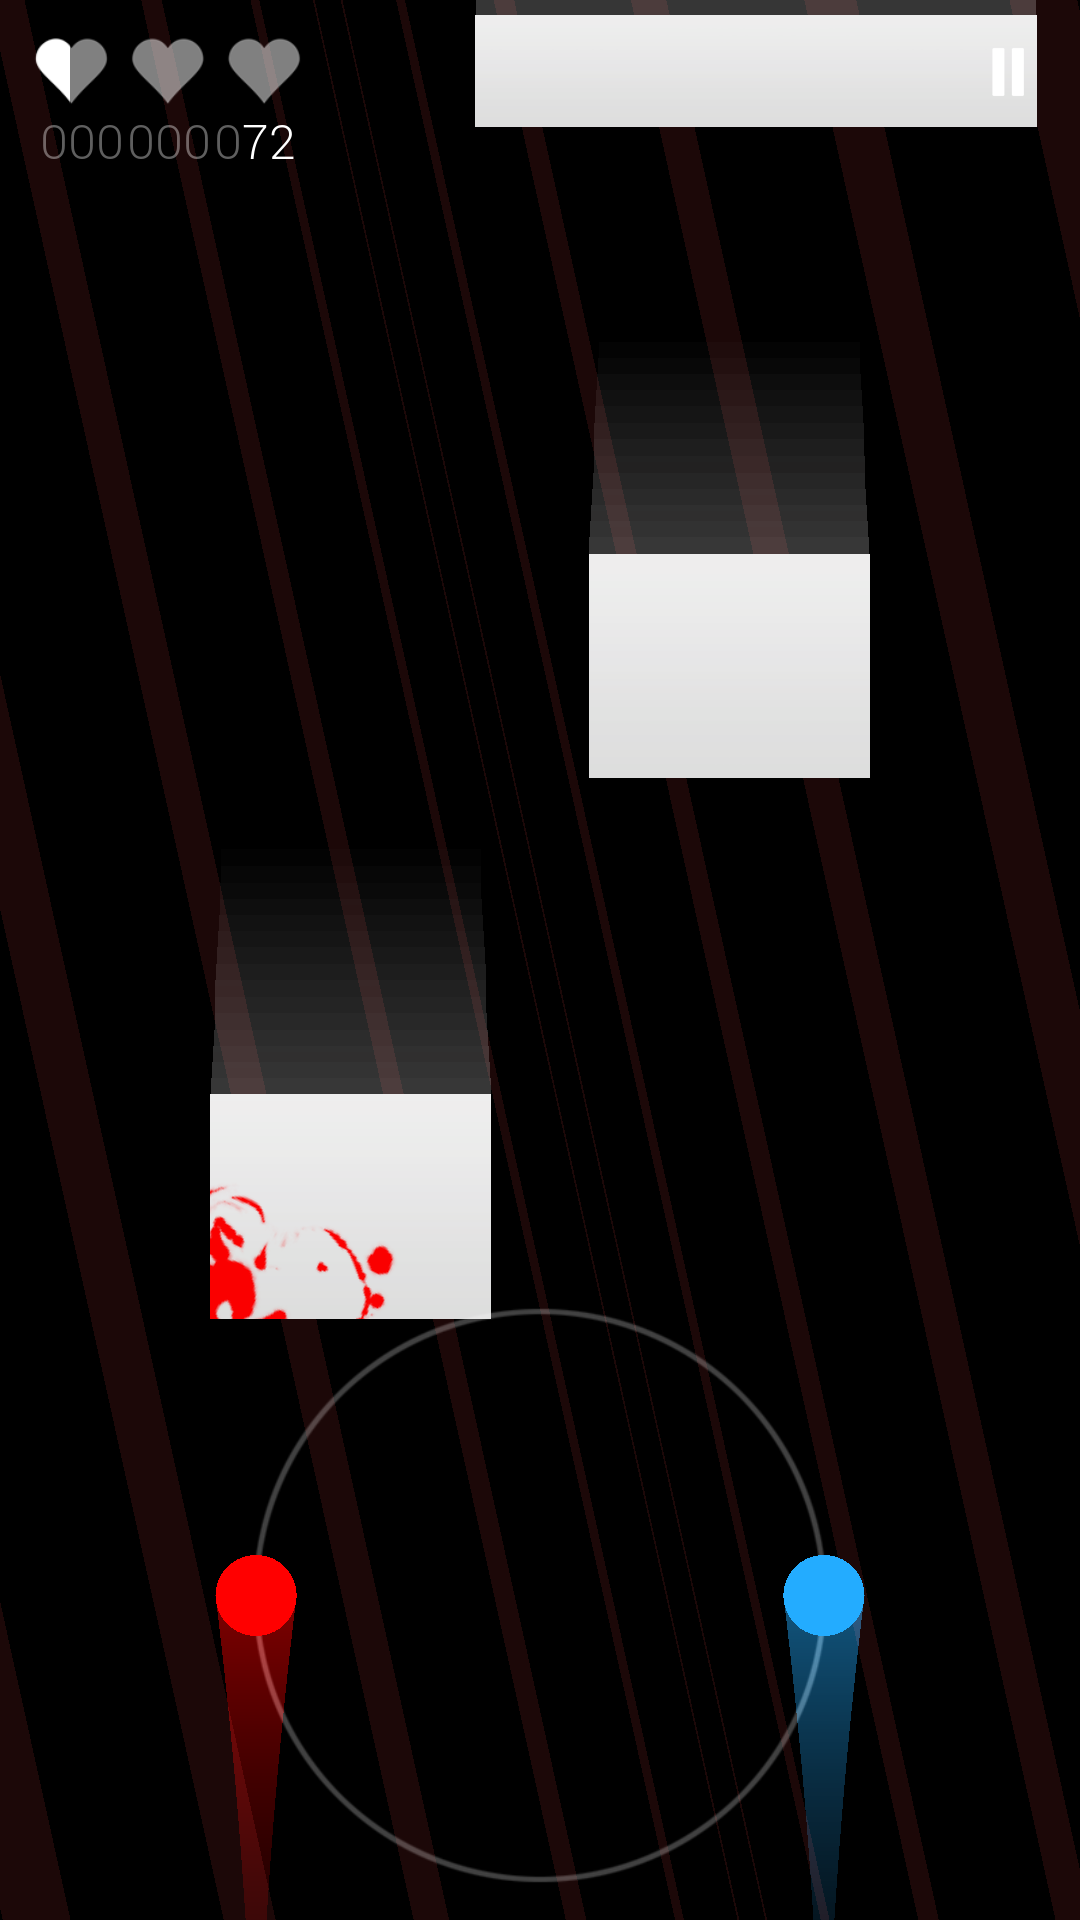
\includegraphics[width=\textwidth]{duet2.png}
		\caption{Screenshot- 2}
	\end{subfigure}
	\caption{App working properly after restrictions}
	\label{fig:duet}
\end{figure}